% Options for packages loaded elsewhere
\PassOptionsToPackage{unicode}{hyperref}
\PassOptionsToPackage{hyphens}{url}
\PassOptionsToPackage{dvipsnames,svgnames,x11names}{xcolor}
%
\documentclass[
  letterpaper,
  DIV=11,
  numbers=noendperiod]{scrartcl}

\usepackage{amsmath,amssymb}
\usepackage{iftex}
\ifPDFTeX
  \usepackage[T1]{fontenc}
  \usepackage[utf8]{inputenc}
  \usepackage{textcomp} % provide euro and other symbols
\else % if luatex or xetex
  \usepackage{unicode-math}
  \defaultfontfeatures{Scale=MatchLowercase}
  \defaultfontfeatures[\rmfamily]{Ligatures=TeX,Scale=1}
\fi
\usepackage{lmodern}
\ifPDFTeX\else  
    % xetex/luatex font selection
\fi
% Use upquote if available, for straight quotes in verbatim environments
\IfFileExists{upquote.sty}{\usepackage{upquote}}{}
\IfFileExists{microtype.sty}{% use microtype if available
  \usepackage[]{microtype}
  \UseMicrotypeSet[protrusion]{basicmath} % disable protrusion for tt fonts
}{}
\makeatletter
\@ifundefined{KOMAClassName}{% if non-KOMA class
  \IfFileExists{parskip.sty}{%
    \usepackage{parskip}
  }{% else
    \setlength{\parindent}{0pt}
    \setlength{\parskip}{6pt plus 2pt minus 1pt}}
}{% if KOMA class
  \KOMAoptions{parskip=half}}
\makeatother
\usepackage{xcolor}
\setlength{\emergencystretch}{3em} % prevent overfull lines
\setcounter{secnumdepth}{-\maxdimen} % remove section numbering
% Make \paragraph and \subparagraph free-standing
\makeatletter
\ifx\paragraph\undefined\else
  \let\oldparagraph\paragraph
  \renewcommand{\paragraph}{
    \@ifstar
      \xxxParagraphStar
      \xxxParagraphNoStar
  }
  \newcommand{\xxxParagraphStar}[1]{\oldparagraph*{#1}\mbox{}}
  \newcommand{\xxxParagraphNoStar}[1]{\oldparagraph{#1}\mbox{}}
\fi
\ifx\subparagraph\undefined\else
  \let\oldsubparagraph\subparagraph
  \renewcommand{\subparagraph}{
    \@ifstar
      \xxxSubParagraphStar
      \xxxSubParagraphNoStar
  }
  \newcommand{\xxxSubParagraphStar}[1]{\oldsubparagraph*{#1}\mbox{}}
  \newcommand{\xxxSubParagraphNoStar}[1]{\oldsubparagraph{#1}\mbox{}}
\fi
\makeatother


\providecommand{\tightlist}{%
  \setlength{\itemsep}{0pt}\setlength{\parskip}{0pt}}\usepackage{longtable,booktabs,array}
\usepackage{calc} % for calculating minipage widths
% Correct order of tables after \paragraph or \subparagraph
\usepackage{etoolbox}
\makeatletter
\patchcmd\longtable{\par}{\if@noskipsec\mbox{}\fi\par}{}{}
\makeatother
% Allow footnotes in longtable head/foot
\IfFileExists{footnotehyper.sty}{\usepackage{footnotehyper}}{\usepackage{footnote}}
\makesavenoteenv{longtable}
\usepackage{graphicx}
\makeatletter
\def\maxwidth{\ifdim\Gin@nat@width>\linewidth\linewidth\else\Gin@nat@width\fi}
\def\maxheight{\ifdim\Gin@nat@height>\textheight\textheight\else\Gin@nat@height\fi}
\makeatother
% Scale images if necessary, so that they will not overflow the page
% margins by default, and it is still possible to overwrite the defaults
% using explicit options in \includegraphics[width, height, ...]{}
\setkeys{Gin}{width=\maxwidth,height=\maxheight,keepaspectratio}
% Set default figure placement to htbp
\makeatletter
\def\fps@figure{htbp}
\makeatother
% definitions for citeproc citations
\NewDocumentCommand\citeproctext{}{}
\NewDocumentCommand\citeproc{mm}{%
  \begingroup\def\citeproctext{#2}\cite{#1}\endgroup}
\makeatletter
 % allow citations to break across lines
 \let\@cite@ofmt\@firstofone
 % avoid brackets around text for \cite:
 \def\@biblabel#1{}
 \def\@cite#1#2{{#1\if@tempswa , #2\fi}}
\makeatother
\newlength{\cslhangindent}
\setlength{\cslhangindent}{1.5em}
\newlength{\csllabelwidth}
\setlength{\csllabelwidth}{3em}
\newenvironment{CSLReferences}[2] % #1 hanging-indent, #2 entry-spacing
 {\begin{list}{}{%
  \setlength{\itemindent}{0pt}
  \setlength{\leftmargin}{0pt}
  \setlength{\parsep}{0pt}
  % turn on hanging indent if param 1 is 1
  \ifodd #1
   \setlength{\leftmargin}{\cslhangindent}
   \setlength{\itemindent}{-1\cslhangindent}
  \fi
  % set entry spacing
  \setlength{\itemsep}{#2\baselineskip}}}
 {\end{list}}
\usepackage{calc}
\newcommand{\CSLBlock}[1]{\hfill\break\parbox[t]{\linewidth}{\strut\ignorespaces#1\strut}}
\newcommand{\CSLLeftMargin}[1]{\parbox[t]{\csllabelwidth}{\strut#1\strut}}
\newcommand{\CSLRightInline}[1]{\parbox[t]{\linewidth - \csllabelwidth}{\strut#1\strut}}
\newcommand{\CSLIndent}[1]{\hspace{\cslhangindent}#1}

\KOMAoption{captions}{tableheading}
\makeatletter
\@ifpackageloaded{caption}{}{\usepackage{caption}}
\AtBeginDocument{%
\ifdefined\contentsname
  \renewcommand*\contentsname{Table of contents}
\else
  \newcommand\contentsname{Table of contents}
\fi
\ifdefined\listfigurename
  \renewcommand*\listfigurename{List of Figures}
\else
  \newcommand\listfigurename{List of Figures}
\fi
\ifdefined\listtablename
  \renewcommand*\listtablename{List of Tables}
\else
  \newcommand\listtablename{List of Tables}
\fi
\ifdefined\figurename
  \renewcommand*\figurename{Figure}
\else
  \newcommand\figurename{Figure}
\fi
\ifdefined\tablename
  \renewcommand*\tablename{Table}
\else
  \newcommand\tablename{Table}
\fi
}
\@ifpackageloaded{float}{}{\usepackage{float}}
\floatstyle{ruled}
\@ifundefined{c@chapter}{\newfloat{codelisting}{h}{lop}}{\newfloat{codelisting}{h}{lop}[chapter]}
\floatname{codelisting}{Listing}
\newcommand*\listoflistings{\listof{codelisting}{List of Listings}}
\makeatother
\makeatletter
\makeatother
\makeatletter
\@ifpackageloaded{caption}{}{\usepackage{caption}}
\@ifpackageloaded{subcaption}{}{\usepackage{subcaption}}
\makeatother

\ifLuaTeX
  \usepackage{selnolig}  % disable illegal ligatures
\fi
\usepackage{bookmark}

\IfFileExists{xurl.sty}{\usepackage{xurl}}{} % add URL line breaks if available
\urlstyle{same} % disable monospaced font for URLs
\hypersetup{
  pdftitle={Coup-Proofing via Capital Relocation},
  colorlinks=true,
  linkcolor={blue},
  filecolor={Maroon},
  citecolor={Blue},
  urlcolor={Blue},
  pdfcreator={LaTeX via pandoc}}


\title{Coup-Proofing via Capital Relocation}
\usepackage{etoolbox}
\makeatletter
\providecommand{\subtitle}[1]{% add subtitle to \maketitle
  \apptocmd{\@title}{\par {\large #1 \par}}{}{}
}
\makeatother
\subtitle{DSAN 6750 / PPOL 6805: GIS for Spatial Data Science}
\author{Jeff Jacobs}
\date{}

\begin{document}
\maketitle


\subsection{Introduction}\label{introduction}

Several previous studies have found robust relationships between spatial
properties of a country's \textbf{capital city} and that country's
propensity for \textbf{conflict} and \textbf{misgovernance}.

Perceptions of this linkage also have an effect on ``coup-proofing''
decisions made by national governments. A recent BBC interview with
Equatorial Guinea's President Teodoro Obiang, for example, highlighted
this as a factor behind his decision to relocate the capital city:

\begin{quote}
It's the remoteness of Oyala that makes it so appealing to President
Obiang. In a rare interview he described how rebels had recently plotted
a seaborne assault on his palace in the current capital, Malabo. `We
need a secure place for my government and for future governments. That's
why we have created Oyala, to guarantee the government of Equatorial
Guinea.' (\citeproc{ref-sackur_equatorial_2012}{Sackur 2012})
\end{quote}

This case is far from exceptional, as an even more recent
\emph{Washington Post} article points out with respect to Myanmar's
decision to move its capital from Yangon to Naypyidaw:

\begin{quote}
Analysts have described the decision as motivated by a desire to secure
the military's seat of power from any threat of protests or invasions.
(\citeproc{ref-berger_myanmars_2021}{Berger 2021})
\end{quote}

Most of these studies, however, are based on observations of
\textbf{conflict events}. In this study, we study the more fundamental
variable of a capital's distance from the \textbf{population centroid}
of the country.

\subsection{Literature Review}\label{literature-review}

Campante, Do, and Guimaraes (\citeproc{ref-campante_capital_2019}{2019})
analyzes the relationship between the location of a \textbf{capital
city} and the degree of conflict and misgovernance in a given country.
Their two key findings are that:

\begin{quote}
Conflict is more likely to emerge (and dislodge incumbents) closer to
the capital
\end{quote}

and

\begin{quote}
Isolated capitals are associated with misgovernance.
\end{quote}

This first finding is illustrated in Figure~\ref{fig-conflict-dist}

\begin{figure}

\centering{

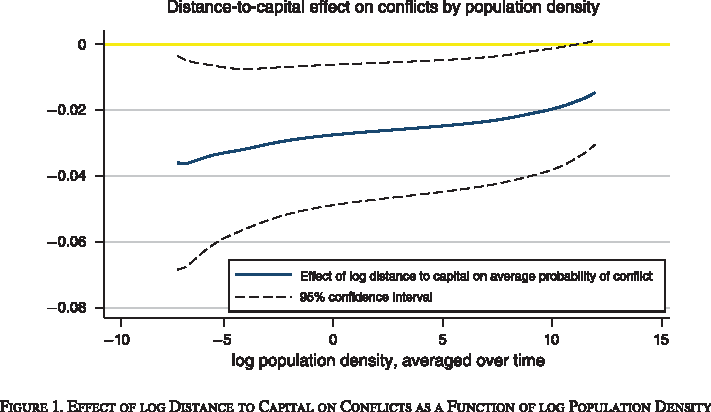
\includegraphics{index_files/mediabag/images/conflict_dist.pdf}

}

\caption{\label{fig-conflict-dist}}

\end{figure}%

\subsection{Methodology}\label{methodology}

The \textbf{population centroids} we use herein might require some
explanation, since the term ``centroid'' can be ambiguous.

Here, the population centroids are drawn from Hall et al.
(\citeproc{ref-hall_population_2019}{2019})

\subsection{Exploratory Data Analysis
(EDA)}\label{exploratory-data-analysis-eda}

Here we plot the base GIS objects we're analyzing: the location of each
\textbf{capital city} (in purple) and each \textbf{population centroid}
(in yellow).

\textsubscript{Source:
\href{https://jpowerj.github.io/gis-manuscript-template/index.qmd.html}{Article
Notebook}}

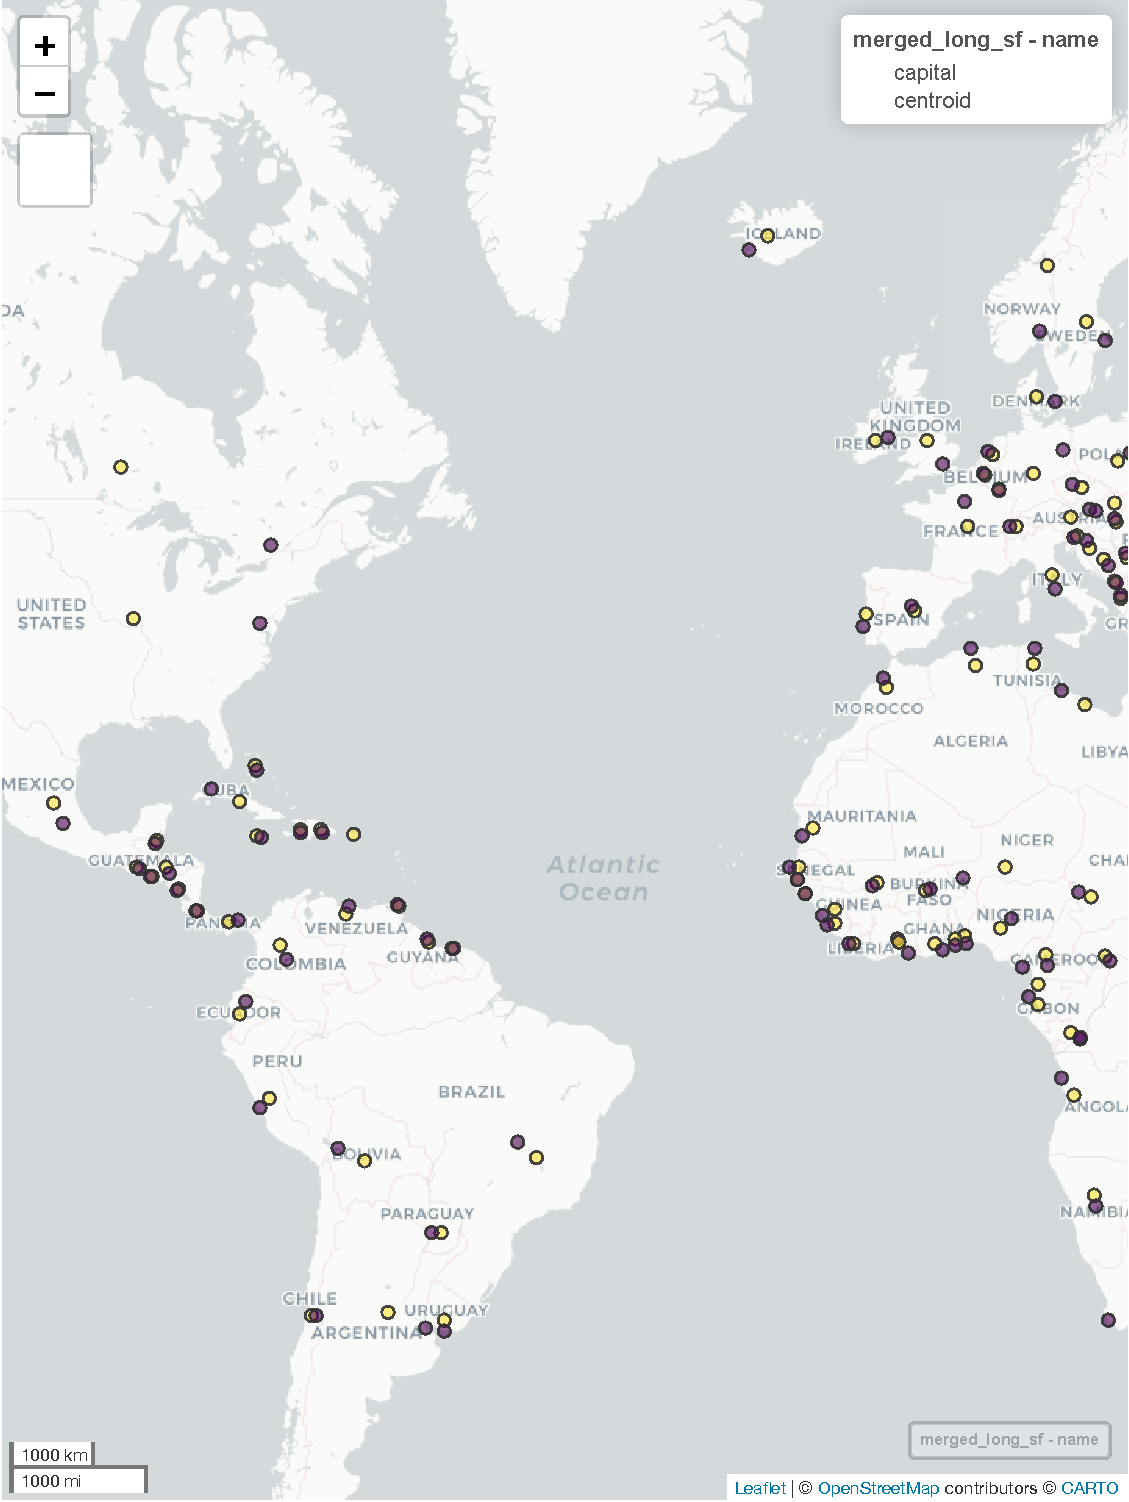
\includegraphics{index_files/figure-pdf/load-eda-1.pdf}

\textsubscript{Source:
\href{https://jpowerj.github.io/gis-manuscript-template/index.qmd.html}{Article
Notebook}}

We then construct an \textbf{area-normalized} measure of
capital-centroid distance \(\text{dist}^{\textsf{AN}}\), using the
formula

\[
\text{dist}^{\textsf{AN}}_i = \text{dist}_i / \sqrt{\text{area}_i}.
\]

A plot of this measure by country looks as follows:

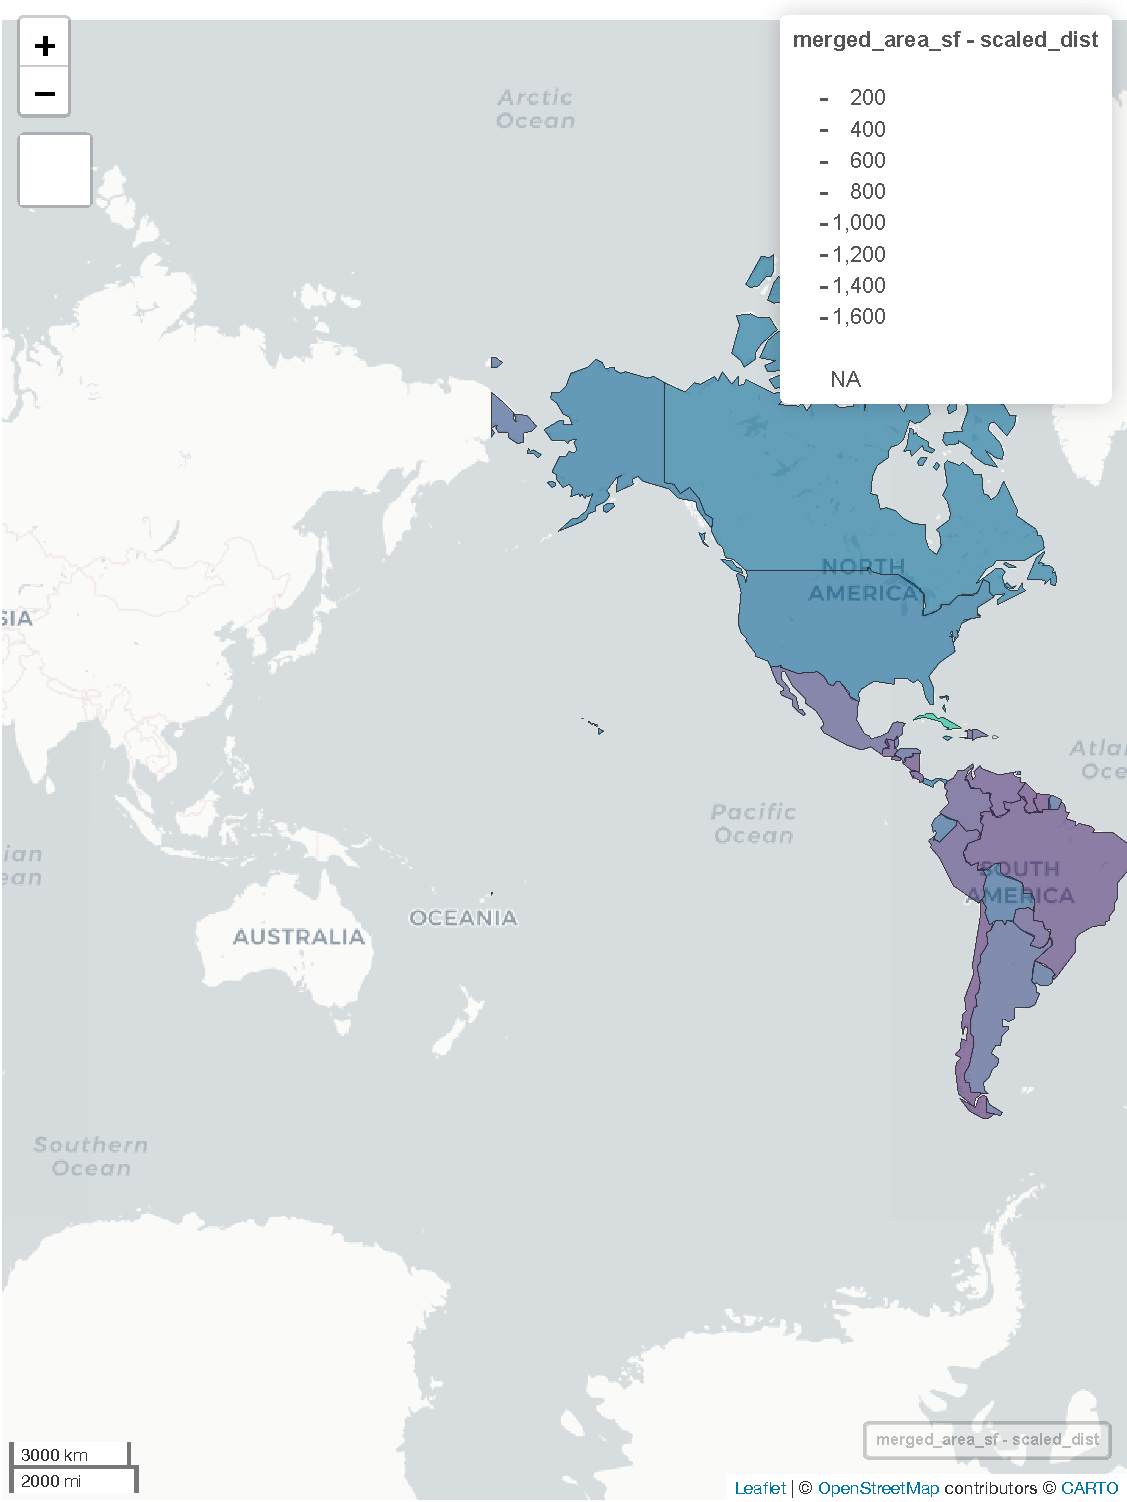
\includegraphics{index_files/figure-pdf/plot-area-1.pdf}

\textsubscript{Source:
\href{https://jpowerj.github.io/gis-manuscript-template/index.qmd.html}{Article
Notebook}}

\subsection{Hypothesis Testing
(Regression)}\label{hypothesis-testing-regression}

\begin{longtable}[]{@{}
  >{\raggedright\arraybackslash}p{(\columnwidth - 26\tabcolsep) * \real{0.1126}}
  >{\raggedright\arraybackslash}p{(\columnwidth - 26\tabcolsep) * \real{0.0315}}
  >{\raggedleft\arraybackslash}p{(\columnwidth - 26\tabcolsep) * \real{0.0405}}
  >{\raggedleft\arraybackslash}p{(\columnwidth - 26\tabcolsep) * \real{0.0225}}
  >{\raggedright\arraybackslash}p{(\columnwidth - 26\tabcolsep) * \real{0.0766}}
  >{\raggedleft\arraybackslash}p{(\columnwidth - 26\tabcolsep) * \real{0.0405}}
  >{\raggedright\arraybackslash}p{(\columnwidth - 26\tabcolsep) * \real{0.0811}}
  >{\raggedleft\arraybackslash}p{(\columnwidth - 26\tabcolsep) * \real{0.0631}}
  >{\raggedleft\arraybackslash}p{(\columnwidth - 26\tabcolsep) * \real{0.0360}}
  >{\raggedleft\arraybackslash}p{(\columnwidth - 26\tabcolsep) * \real{0.0586}}
  >{\raggedleft\arraybackslash}p{(\columnwidth - 26\tabcolsep) * \real{0.0541}}
  >{\raggedright\arraybackslash}p{(\columnwidth - 26\tabcolsep) * \real{0.1396}}
  >{\raggedright\arraybackslash}p{(\columnwidth - 26\tabcolsep) * \real{0.1216}}
  >{\raggedright\arraybackslash}p{(\columnwidth - 26\tabcolsep) * \real{0.1216}}@{}}
\toprule\noalign{}
\begin{minipage}[b]{\linewidth}\raggedright
geounit
\end{minipage} & \begin{minipage}[b]{\linewidth}\raggedright
iso\_a3
\end{minipage} & \begin{minipage}[b]{\linewidth}\raggedleft
OBJECTID
\end{minipage} & \begin{minipage}[b]{\linewidth}\raggedleft
ID\_0
\end{minipage} & \begin{minipage}[b]{\linewidth}\raggedright
NAME\_ENGLI
\end{minipage} & \begin{minipage}[b]{\linewidth}\raggedleft
OUT\_FLAG
\end{minipage} & \begin{minipage}[b]{\linewidth}\raggedright
NAME
\end{minipage} & \begin{minipage}[b]{\linewidth}\raggedleft
dist
\end{minipage} & \begin{minipage}[b]{\linewidth}\raggedleft
area
\end{minipage} & \begin{minipage}[b]{\linewidth}\raggedleft
scaled\_dist
\end{minipage} & \begin{minipage}[b]{\linewidth}\raggedleft
total\_score
\end{minipage} & \begin{minipage}[b]{\linewidth}\raggedright
geometry
\end{minipage} & \begin{minipage}[b]{\linewidth}\raggedright
centroid
\end{minipage} & \begin{minipage}[b]{\linewidth}\raggedright
capital
\end{minipage} \\
\midrule\noalign{}
\endhead
\bottomrule\noalign{}
\endlastfoot
Tanzania & TZA & 227 & 227 & Tanzania & 0 & Dar es Salaam & 324758.1
{[}m{]} & 885800 & 345.0580 {[}m{]} & 0.007 & MULTIPOLYGON (((33.90371
-0\ldots{} & POINT (36.5813 -5.612844) & POINT (39.2664 -6.798067) \\
Canada & CAN & 42 & 42 & Canada & 0 & Ottawa & 1410811.7 {[}m{]} &
8788700 & 475.8902 {[}m{]} & 0.001 & MULTIPOLYGON (((-122.84 49,\ldots{}
& POINT (-92.673 51.33108) & POINT (-75.70196 45.41864) \\
United States of America & USA & 244 & 244 & United States & 0 &
Washington, D.C. & 1227411.4 {[}m{]} & 9147420 & 405.8269 {[}m{]} &
0.022 & MULTIPOLYGON (((-122.84 49,\ldots{} & POINT (-91.24719 39.43566)
& POINT (-77.01136 38.9015) \\
Kazakhstan & KAZ & 117 & 117 & Kazakhstan & 0 & Nur-Sultan & 227074.6
{[}m{]} & 2699700 & 138.2009 {[}m{]} & 0.010 & MULTIPOLYGON (((87.35997
49\ldots{} & POINT (69.7252 49.45229) & POINT (71.42777 51.18113) \\
Uzbekistan & UZB & 246 & 246 & Uzbekistan & 0 & Tashkent & 168011.1
{[}m{]} & 440653 & 253.0985 {[}m{]} & 0.005 & MULTIPOLYGON (((55.96819
41\ldots{} & POINT (67.77264 40.30358) & POINT (69.26882 41.30383) \\
Papua New Guinea & PNG & 175 & 175 & Papua New Guinea & 0 & Port Moresby
& 289887.1 {[}m{]} & 452860 & 430.7714 {[}m{]} & 0.025 & MULTIPOLYGON
(((141.0002 -2\ldots{} & POINT (146.2921 -7.014699) & POINT (147.1925
-9.464708) \\
\end{longtable}

\textsubscript{Source:
\href{https://jpowerj.github.io/gis-manuscript-template/index.qmd.html}{Article
Notebook}}

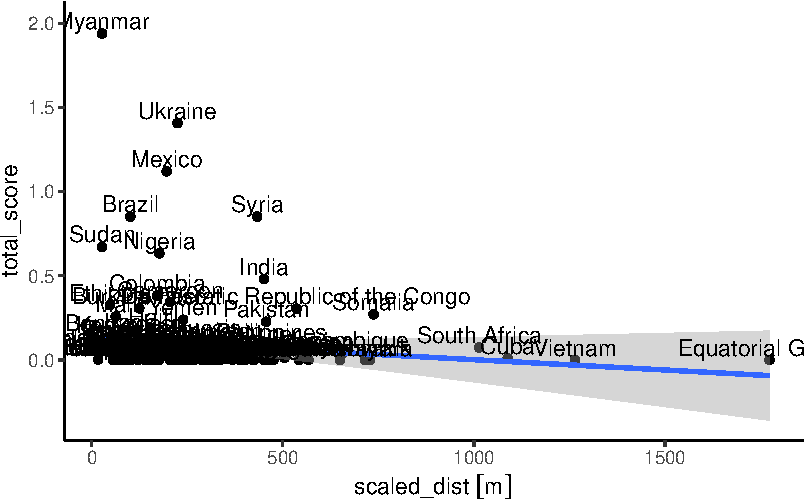
\includegraphics{index_files/figure-pdf/unnamed-chunk-5-1.pdf}

\textsubscript{Source:
\href{https://jpowerj.github.io/gis-manuscript-template/index.qmd.html}{Article
Notebook}}

\subsection{Discussion}\label{discussion}

\subsection{Conclusion}\label{conclusion}

Our evidence indicates that the spatial dynamics of \textbf{conflict}
differ from the spatial dynamics of \textbf{misgovernance}. Whereas

\phantomsection\label{refs}
\begin{CSLReferences}{1}{0}
\bibitem[\citeproctext]{ref-berger_myanmars_2021}
Berger, Miriam. 2021. {``Myanmar's Military Built a New Capital as a
Haven for Power. {Other} Countries Have Tried That, Too.''}
\emph{Washington Post}, February.
\url{https://www.washingtonpost.com/world/2021/02/06/myanmars-military-built-new-capital-haven-power-other-countries-have-tried-that-too/}.

\bibitem[\citeproctext]{ref-campante_capital_2019}
Campante, Filipe R., Quoc-Anh Do, and Bernardo Guimaraes. 2019.
{``Capital {Cities}, {Conflict}, and {Misgovernance}.''} \emph{American
Economic Journal: Applied Economics} 11 (3): 298--337.
\url{https://doi.org/10.1257/app.20170111}.

\bibitem[\citeproctext]{ref-hall_population_2019}
Hall, Ola, Maria Francisca Archila Bustos, Niklas Boke Olén, and Thomas
Niedomysl. 2019. {``Population Centroids of the World Administrative
Units from Nighttime Lights 1992-2013.''} \emph{Scientific Data} 6 (1):
235. \url{https://doi.org/10.1038/s41597-019-0250-z}.

\bibitem[\citeproctext]{ref-sackur_equatorial_2012}
Sackur, Stephen. 2012. {``Equatorial {Guinea}: {Obiang}'s Future
Capital, {Oyala}.''} \emph{BBC News}, December.
\url{https://www.bbc.com/news/magazine-20731448}.

\end{CSLReferences}




\end{document}
